\documentclass[
  11pt,
  letterpaper,
   addpoints,
   %answers
  ]{exam}

\usepackage{../exercise-preamble}
\usepackage{float}
\usepackage[most]{tcolorbox}

\begin{document}

\noindent
\begin{minipage}{0.47\textwidth}
\includegraphics[width=\textwidth]{../fcfm_die}
\end{minipage}
\begin{minipage}{0.53\textwidth}
\begin{center} 
\large\textbf{Circuitos Eléctricos Analógicos} (EL3202) \\
\large\textbf{Control 1} \\
\normalsize Prof Patricio Mendoza \\
\normalsize Prof Aux  Renato Planas , Erik Sáez Aravena
\end{center}
\end{minipage}

\begin{tcolorbox}[colback=gray!10!white,colframe=black!80!white,title=Instrucciones]
Dispone de 1 hora y media para contestar el control. No se permite el uso de calculadoras ni teléfonos. Recuerde escribir su nombre y RUT en todas las hojas. La sospecha de copia será sancionada.
\end{tcolorbox}

\begin{questions}
  %%%%%%%%%%%%%%%%%%%%%%%%%%%
  \question P1
%--------------------------
  \question Resuelva lo siguiente:
  \begin{parts}
    \part \textbf{[3 Puntos]} Dado el circuito visto en la Figura \ref{Figura_01}, calcule el punto de operación que pasa por el diodo $D_1$ ($V_{in} = 12$ V, $R_1= 10$ k$\Omega$, $R_2 = 5$ k$\Omega$, $R_3 = 35$ k$\Omega$, y $R_4= 50$ k$\Omega$) y grafique la recta de carga del circuito.
  \begin{figure}[H]
    \centering
    \begin{circuitikz}[scale=1.2, transform shape]
      % Voltage source
      \draw (0,2) to[battery1, l=$V_{in}$] (0,0);
      % R1
      \draw (0,2) to[R, l=$R_1$] (2,2);
      % R3
      \draw (2,2) to[R, l=$R_3$] (4,2);
      % R2
      \draw (2,2) to[R, l=$R_2$] (2,0);
      % Diode D2
      \draw (4,2) to[empty diode, l=$D_2$] (4,0);
      % R4
      \draw (4,2) to[R, l=$R_4$] (6,2);
      \draw (6,2) -- (6,0);
      % Ground connections
      \draw (0,0) -- (6,0);
      \draw (3,0) node[ground]{};
    \end{circuitikz}
    \caption{Circuito con diodo.}
    \label{Figura_01}
  \end{figure}
  Para esto asuma que la curva característica (v-i) del diodo está dada por la Figura \ref{Figura_2}.
    \begin{figure}[H]
    \centering
    \includegraphics[width=0.6\textwidth]{Control_01_2}
    \caption{Curva característica del diodo.}
    \label{Figura_2}
  \end{figure}
    \part \textbf{[3 Puntos]} Asuma $V_\gamma = 0.7$ V para cada diodo en el circuito en la Figura \ref{Fig2}. Grafique $v_O$ versus $v_I$ para $-10 \leq v_I \leq +10$ V.
  \begin{figure}[H]
      \centering
      \begin{circuitikz}[scale=1.0, transform shape]
        % Nodo central superior
        \coordinate (top) at (0,2);
        % Nodo central inferior
        \coordinate (bottom) at (0,-2);
        % Nodo izquierdo
        \coordinate (left) at (-2,0);
        % Nodo derecho
        \coordinate (right) at (2,0);
        
        % Entrada vI
        \draw (left) to[short, o-*] ++(-0.5,0) node[anchor=east] {$v_I$};
        
        % Diodos formando el puente
        \draw (top) to[D, l=$D_1$] (left);
        \draw (top) to[D, l=$D_2$] (right);
        \draw (right) to[D, l=$D_4$] (bottom);
        \draw (left) to[D, l=$D_3$] (bottom);
        
        % Resistencia superior a +10V
        \draw (top) to[R, l=$10\,k\Omega$] ++(0,1.5) to[short, -o] ++(0,0.3) node[anchor=south] {$+10\,V$};
        
        % Resistencia inferior a -10V
        \draw (bottom) to[R, l=$10\,k\Omega$] ++(0,-1.5) to[short, -o] ++(0,-0.3) node[anchor=north] {$-10\,V$};
        
        % Resistencia de carga y salida vO
        \draw (right) to[short, *-] ++(0.5,0) coordinate (out);
        \draw (out) to[R, l=$10\,k\Omega$] ++(0,-2) node[ground] {};
        \draw (out) to[short, -o] ++(0.8,0) node[anchor=west] {$v_O$};
      \end{circuitikz}
      \caption{Circuito con diodos.}
      \label{Fig2}
  \end{figure}
  \textit{Hint: Puede ser util analizar el caso en que $D_1$ y $D_4$ se encuentran apagados.}
  \end{parts}
  %--------------------------
  \begin{solution}
    \subsection*{Resolución a)}
    Dado que buscamos obtener el punto de operación en los dos puntos de interés, analizamos los siguientes casos:
    \begin{itemize}
      \item \textbf{Diodo $D_1$ en cortocircuito:} Dado que tenemos el diodo en cortocircuito, el circuito será:
      \begin{figure}[H]
        \centering
        \begin{circuitikz}[scale=1.2, transform shape]
          % Voltage source
          \draw (0,2) to[battery1, l=$V_{in}$] (0,0);
          % R1
          \draw (0,2) to[R, l=$R_1$] (2,2);
          % R3
          \draw (2,2) to[R, l=$R_3$] (4,2);
          % R2
          \draw (2,2) to[R, l=$R_2$] (2,0);
          % Short circuit for D1
          \draw (4,2) -- (4,0);
          % R4
          \draw (4,2) to[R, l=$R_4$] (6,2);
          \draw (6,2) -- (6,0);
          % Ground connections
          \draw (0,0) -- (6,0);
          \draw (3,0) node[ground]{};
        \end{circuitikz}
      \end{figure}
      Luego tenemos un cortocircuito en paralelo con $R_4$, por lo tanto, $R_4$ no influye en el circuito, por lo que:
      \begin{figure}[H]
        \centering
        \begin{circuitikz}[scale=1.2, transform shape]
          % Voltage source
          \draw (0,2) to[battery1, l=$V_{in}$] (0,0);
          % R1
          \draw (0,2) to[R, l=$R_1$] (2,2);
          % R3
          \draw (2,2) to[R, l=$R_3$] (4,2);
          % R2
          \draw (2,2) to[R, l=$R_2$] (2,0);
          % Short circuit for D1
          \draw (4,2) -- (4,0);
          % Ground connections
          \draw (0,0) -- (4,0);
          \draw (2,0) node[ground]{};
        \end{circuitikz}
      \end{figure}
      Por lo que nos interesa el voltaje en $R_{3}$. Podemos plantear las ecuaciones por análisis de mallas. Sea $i_1$ la corriente que circula por $R_1$ y $R_2$, e $i_2$ la corriente que circula por $R_3$:
      
      \textbf{Malla 1} (malla izquierda):
      \begin{equation}
        -V_{in} + i_1 R_1 + (i_1 - i_2) R_2 = 0
      \end{equation}
      
      \textbf{Malla 2} (malla derecha):
      \begin{equation}
        (i_2 - i_1) R_2 + i_2 R_3 = 0
      \end{equation}
      
      Expandiendo las ecuaciones con los valores dados:
      \begin{align}
        -12 + i_1 \cdot 10\text{k} + (i_1 - i_2) \cdot 5\text{k} &= 0 \\
        (i_2 - i_1) \cdot 5\text{k} + i_2 \cdot 35\text{k} &= 0
      \end{align}
      
      Simplificando la primera ecuación:
      \begin{align}
        -12 + 10\text{k} \cdot i_1 + 5\text{k} \cdot i_1 - 5\text{k} \cdot i_2 &= 0 \\
        -12 + 15\text{k} \cdot i_1 - 5\text{k} \cdot i_2 &= 0 \\
        15\text{k} \cdot i_1 - 5\text{k} \cdot i_2 &= 12
      \end{align}
      
      Simplificando la segunda ecuación:
      \begin{align}
        5\text{k} \cdot i_2 - 5\text{k} \cdot i_1 + 35\text{k} \cdot i_2 &= 0 \\
        -5\text{k} \cdot i_1 + 40\text{k} \cdot i_2 &= 0 \\
        5\text{k} \cdot i_1 &= 40\text{k} \cdot i_2 \\
        i_1 &= 8 \cdot i_2
      \end{align}
      
      Sustituyendo $i_1 = 8 \cdot i_2$ en la primera ecuación:
      \begin{align}
        15\text{k} \cdot (8 \cdot i_2) - 5\text{k} \cdot i_2 &= 12 \\
        120\text{k} \cdot i_2 - 5\text{k} \cdot i_2 &= 12 \\
        115\text{k} \cdot i_2 &= 12 \\
        i_2 &= \frac{12}{115\text{k}} = \frac{12}{115000} = 0.1043 \text{ mA} \approx 0.10 \text{ mA}
      \end{align}
      
      Y por lo tanto:
      \begin{equation}
        i_1 = 8 \cdot 0.10 \text{ mA} = 0.80 \text{ mA}
      \end{equation}
      
      Por lo que el voltaje en $R_3$ es:
      \begin{equation}
        V_{R_3} = R_3 \cdot i_2 = 35 \text{ k}\Omega \cdot 0.10 \text{ mA} = 3.5 \text{ V}
      \end{equation}
      Por lo tanto, nuestro primer punto de operación es:
      \begin{equation}
        \boxed{(V_{D_1}, I_{D_1}) = (0 \text{ V}, 0.10 \text{ mA})}
      \end{equation}
      \item \textbf{Diodo $D_1$ en circuito abierto:} Dado que tenemos el diodo en circuito abierto, el circuito será:
      \begin{figure}[H]
        \centering
        \begin{circuitikz}[scale=1.2, transform shape]
          % Voltage source
          \draw (0,2) to[battery1, l=$V_{in}$] (0,0);
          % R1
          \draw (0,2) to[R, l=$R_1$] (2,2);
          % R3
          \draw (2,2) to[R, l=$R_3$] (4,2);
          % R2
          \draw (2,2) to[R, l=$R_2$] (2,0);
          % Open circuit for D1
          \draw (4,2) to[open, l=$D_1$] (4,0);
          % R4
          \draw (4,2) to[R, l=$R_4$] (6,2);
          \draw (6,2) -- (6,0);
          % Ground connections
          \draw (0,0) -- (6,0);
          \draw (3,0) node[ground]{};
          % Node labels
          \node at (0,2) [circ, label=above:$A$] {};
          \node at (2,2) [circ, label=above:$B$] {};
          \node at (4,2) [circ, label=above:$C$] {};
          \node at (6,2) [circ, label=above:$D$] {};
          \node at (2,0) [circ, label=below:$E$] {};
     
        \end{circuitikz}
      \end{figure}
Las corrientes serán:
\begin{align}
  i_{AB} = i_{BC} + i_{BE} \\
  i_{BC} = i_{CD}
\end{align}
Reemplazando las corrientes por las tensiones y resistencias:
\begin{align}
  \frac{V_{in} - V_B}{R_1} = \frac{V_B - V_C}{R_3} + \frac{V_B - V_E}{R_2} \\
  \frac{V_B - V_C}{R_3} = \frac{V_C - V_D}{R_4}
\end{align}
Dado que $V_E = 0$ V y $V_D = 0$ V, el sistema de ecuaciones queda con los valores actualizados:
\begin{align}
  \frac{12 - V_B}{10 \text{ k}\Omega} = \frac{V_B - V_C}{35 \text{ k}\Omega} + \frac{V_B}{5 \text{ k}\Omega} \\
  \frac{V_B - V_C}{35 \text{ k}\Omega} = \frac{V_C}{50 \text{ k}\Omega}
\end{align}

Desarrollando la primera ecuación:
\begin{align}
  \frac{12 - V_B}{10} &= \frac{V_B - V_C}{35} + \frac{V_B}{5} \\
  \frac{12 - V_B}{10} &= \frac{V_B - V_C}{35} + \frac{7V_B}{35} \\
  \frac{12 - V_B}{10} &= \frac{V_B - V_C + 7V_B}{35} \\
  \frac{12 - V_B}{10} &= \frac{8V_B - V_C}{35}
\end{align}

Multiplicando cruzado:
\begin{equation}
  35(12 - V_B) = 10(8V_B - V_C)
\end{equation}
\begin{equation}
  420 - 35V_B = 80V_B - 10V_C
\end{equation}
\begin{equation}
  420 = 115V_B - 10V_C \quad \text{...(1)}
\end{equation}

De la segunda ecuación:
\begin{align}
  \frac{V_B - V_C}{35} &= \frac{V_C}{50} \\
  50(V_B - V_C) &= 35V_C \\
  50V_B - 50V_C &= 35V_C \\
  50V_B &= 85V_C \\
  V_B &= 1.7V_C \quad \text{...(2)}
\end{align}

Sustituyendo (2) en (1):
\begin{align}
  420 &= 115(1.7V_C) - 10V_C \\
  420 &= 195.5V_C - 10V_C \\
  420 &= 185.5V_C \\
  V_C &= \frac{420}{185.5} = 2.26 \text{ V}
\end{align}

Por lo tanto:
\begin{equation}
  V_B = 1.7 \times 2.26 = 3.84 \text{ V}
\end{equation}

El voltaje en el diodo $D_1$ es:
\begin{equation}
  V_{D_1} = V_C - V_D = 2.26 \text{ V} - 0 \text{ V} = 2.26 \text{ V}
\end{equation}

Nuestro segundo punto de operación es:
\begin{equation}
  \boxed{(V_{D_1}, I_{D_1}) = (2.26 \text{ V}, 0 \text{ mA})}
\end{equation}
    \end{itemize}

  Finalmente, la intersección con la curva del diodo nos da el punto de operación buscado:
   \begin{figure}[H]
    \centering
    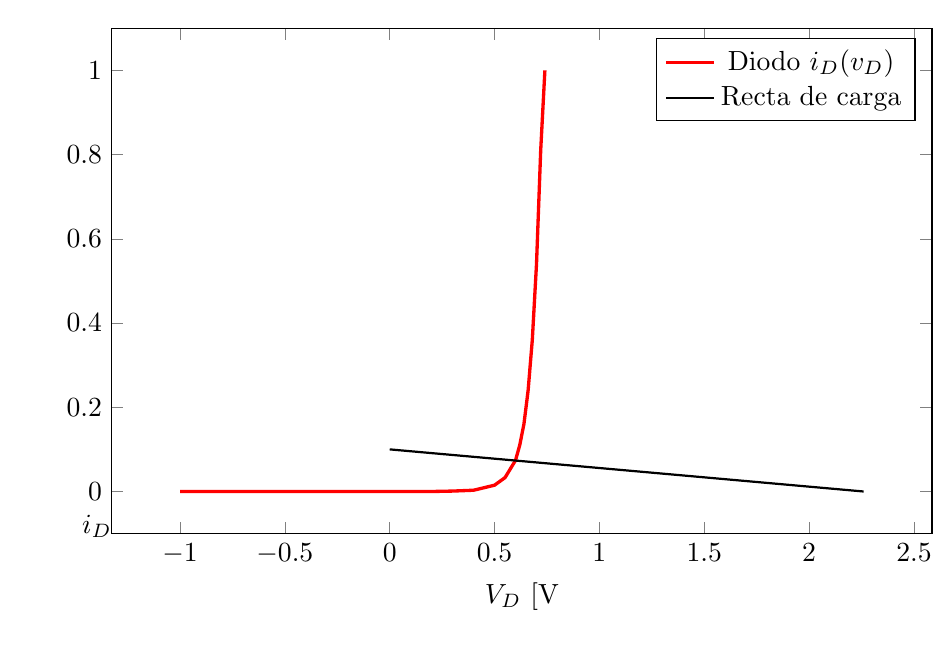
\begin{tikzpicture}
      \begin{axis}[
        width=12cm,
        height=8cm,
        xlabel=$V_D$ [V],
        ylabel=$i_D$ [mA],
        xmin=-1, 
        xmax=3,
        ymin=0, 
        ymax=1,
        xtick={-1,0,0.5,1,1.5,2,2.26,2.5,3},
        ytick={0, 0.1, 0.2, 0.3, 0.4, 0.5, 0.6, 0.7, 0.8, 0.9, 1},
        grid=major,
        grid style={dashed, gray!30},
        legend style={at={(0.35,0.98)}, anchor=north west},
        axis lines=left,
        clip=false,
        enlarge x limits=false,
        enlarge y limits=false,
        width=12cm
      ]
      % Curva del diodo (solo los puntos relevantes para el rango)
      \addplot[red, very thick] coordinates {
        (-1,0) (0,0) (0.1,0.000) (0.2,0.000) (0.3,0.001) (0.4,0.003) 
        (0.5,0.015) (0.55,0.033) (0.6,0.074) (0.62,0.11) (0.64,0.16)
        (0.66,0.24) (0.68,0.36) (0.7,0.54) (0.72,0.81) (0.74,1.0)
      };
      \addlegendentry{Diodo $i_D(v_D)$}
      % Recta de carga (conectando los dos puntos de operacion)
      \addplot[black, thick] coordinates {
        (0, 0.10) (2.26, 0)
      };
      \addlegendentry{Recta de carga}

      \end{axis}
    \end{tikzpicture}
  \end{figure}
  De esta manera, el punto de operación real es:
  \begin{equation}
    \boxed{(V_{D_1}, I_{D_1}) \approx (0.64 \text{ V}, 0.09 \text{ mA})}
  \end{equation}
  \subsection*{Resolución b)}
  
  Para analizar el circuito de la Figura \ref{Fig2}, debemos identificar qué diodos conducen para cada valor de $v_I$. El circuito consiste en un puente de diodos con resistencias de pull-up (+10 V) y pull-down (-10 V), más una resistencia de carga a tierra.
  
  \subsubsection*{Identificación de nodos}
  Llamemos:
  \begin{itemize}
    \item Nodo superior (top): conexión entre $D_1$, $D_2$ y la resistencia a +10 V
    \item Nodo inferior (bottom): conexión entre $D_3$, $D_4$ y la resistencia a -10 V
    \item Nodo izquierdo (left): $v_I$
    \item Nodo derecho (right): $v_O$
  \end{itemize}
  
  \subsubsection*{Análisis por casos}
  
  \textbf{Caso 1: $v_I$ muy positivo (mayor que $v_O + V_\gamma$)}
  
  Cuando $v_I$ es suficientemente positivo, intentará hacer que el nodo izquierdo tenga potencial alto. Los diodos $D_2$ y $D_3$ conducirán:
  \begin{itemize}
    \item $D_2$ conduce: conecta el nodo top con el nodo derecho ($v_O$)
    \item $D_3$ conduce: conecta el nodo izquierdo ($v_I$) con el nodo bottom
    \item $D_1$ y $D_4$ están en corte
  \end{itemize}
  
  El circuito equivalente es:
  \begin{figure}[H]
      \centering
      \begin{circuitikz}[scale=1.2, transform shape]
        % Fuente +10V con resistencia
        \draw (0,3) node[anchor=south] {$+10\,V$} to[short, o-] (0,2.5);
        \draw (0,2.5) to[R, l=$10\,k\Omega$, i=$i_1$] (0,1);
        \draw (0,1) to[short, -o] (0,0.7) node[anchor=south] {$v_O + 0.7$};
        
        % Nodo vO
        \draw (0,0) to[short, *-o] (1,0) node[anchor=west] {$v_O$};
        \draw (0,0) to[R, l=$10\,k\Omega$, i=$i_2$] (0,-2) node[ground] {};
        
        % Entrada vI conectada a -10V
        \draw (-3,0) node[anchor=east] {$v_I$} to[short, o-] (-2.5,0);
        \draw (-2.5,0) to[short] (-2.5,-0.7) node[anchor=north] {$v_I - 0.7$};
        \draw (-2.5,-1) to[R, l=$10\,k\Omega$, i=$i_3$] (-2.5,-2.5);
        \draw (-2.5,-2.5) to[short, -o] (-2.5,-3) node[anchor=north] {$-10\,V$};
      \end{circuitikz}
      \caption{Circuito equivalente cuando $D_2$ y $D_3$ conducen.}
  \end{figure}
  
  Aplicando divisor de tensión entre +10 V y tierra a través de las dos resistencias de 10 k$\Omega$:
  \begin{equation}
    v_O = \frac{(+10 - 0.7) \cdot 10\text{ k}\Omega}{10\text{ k}\Omega + 10\text{ k}\Omega} = \frac{9.3}{2} = 4.65 \text{ V}
  \end{equation}
  
  Este resultado es válido mientras $v_I > v_O + V_\gamma = 4.65 + 0.7 = 5.35$ V.
  
  \textbf{Caso 2: $v_I$ muy negativo (menor que $v_O - V_\gamma$)}
  
  Cuando $v_I$ es suficientemente negativo, los diodos $D_1$ y $D_4$ conducirán:
  \begin{itemize}
    \item $D_1$ conduce: conecta el nodo izquierdo ($v_I$) con el nodo top
    \item $D_4$ conduce: conecta el nodo derecho ($v_O$) con el nodo bottom
    \item $D_2$ y $D_3$ están en corte
  \end{itemize}
  
  Por simetría del circuito, aplicando el mismo análisis:
  \begin{equation}
    v_O = \frac{(-10 + 0.7) \cdot 10\text{ k}\Omega}{10\text{ k}\Omega + 10\text{ k}\Omega} = \frac{-9.3}{2} = -4.65 \text{ V}
  \end{equation}
  
  Este resultado es válido mientras $v_I < v_O - V_\gamma = -4.65 - 0.7 = -5.35$ V.
  
  \textbf{Caso 3: Región intermedia ($-5.35 \text{ V} < v_I < 5.35 \text{ V}$)}
  
  En esta región, ningún par de diodos conduce completamente. El circuito está en una zona de transición donde todos los diodos están en corte. En esta situación, la resistencia de carga a tierra determina que:
  \begin{equation}
    v_O = 0 \text{ V}
  \end{equation}
  
  \textbf{Resumen de la función de transferencia:}
  \begin{equation}
    v_O = \begin{cases}
      +4.65 \text{ V} & \text{si } v_I > +5.35 \text{ V} \\
      0 \text{ V} & \text{si } -5.35 \text{ V} \leq v_I \leq +5.35 \text{ V} \\
      -4.65 \text{ V} & \text{si } v_I < -5.35 \text{ V}
    \end{cases}
  \end{equation}
  
  \textbf{Gráfica $v_O$ vs $v_I$:}
  \begin{figure}[H]
    \centering
    \begin{tikzpicture}
      \begin{axis}[
        width=12cm,
        height=8cm,
        xlabel=$v_I$ [V],
        ylabel=$v_O$ [V],
        xmin=-11,
        xmax=11,
        ymin=-6,
        ymax=6,
        xtick={-10,-5.35,0,5.35,10},
        ytick={-4.65,0,4.65},
        grid=major,
        grid style={dashed, gray!30},
        axis lines=middle,
        axis line style={-stealth},
        every axis x label/.style={at={(ticklabel* cs:1.0)}, anchor=west},
        every axis y label/.style={at={(ticklabel* cs:1.0)}, anchor=south},
        clip=false
      ]
      % Línea horizontal inferior
      \addplot[blue, very thick] coordinates {(-10, -4.65) (-5.35, -4.65)};
      % Línea horizontal en cero
      \addplot[blue, very thick] coordinates {(-5.35, 0) (5.35, 0)};
      % Línea horizontal superior
      \addplot[blue, very thick] coordinates {(5.35, 4.65) (10, 4.65)};
      
      % Transiciones verticales (discontinuidades)
      \addplot[blue, very thick, dashed] coordinates {(-5.35, -4.65) (-5.35, 0)};
      \addplot[blue, very thick, dashed] coordinates {(5.35, 0) (5.35, 4.65)};
      
      % Líneas de referencia
      \addplot[dashed, gray] coordinates {(-5.35, -6) (-5.35, 6)};
      \addplot[dashed, gray] coordinates {(5.35, -6) (5.35, 6)};
      \addplot[dashed, gray] coordinates {(-11, 4.65) (11, 4.65)};
      \addplot[dashed, gray] coordinates {(-11, -4.65) (11, -4.65)};
      
      % Puntos de transición
      \addplot[only marks, mark=*, mark size=3pt, color=blue] coordinates {(-5.35, -4.65) (-5.35, 0) (5.35, 0) (5.35, 4.65)};
      
      \end{axis}
    \end{tikzpicture}
    \caption{Gráfica de $v_O$ versus $v_I$ (circuito limitador).}
  \end{figure}
  
  \boxed{
  \text{El circuito actúa como un limitador doble que mantiene } v_O \text{ en } \pm 4.65 \text{ V o 0 V}
  }
  %--------------------------
  \end{solution}
\end{questions}
\end{document}